\chapter{Projektformulering}
\section{Indledning}
I dette projektet skal der udvikles en slikkanon til spillet Goofy Candygun 3000. Denne slikkanon skal kunne skyde med slik. Dette kunne for eksempel være M\&M’s eller Skittle’s.

Goofy Candygun 3000 er et spil til to personer. Spillet går ud på at opnå flest point ved at ramme et mål. Hver spiller får et bestemt antal skud. Efter skuddene er opbrugt, er vinderen den spiller med flest point.

Det endelige produkt omfatter:
\begin{itemize}
	\item{En brugergrænseflade, hvor spilstatistikker fremvises til deltagerne. Dette er blandt andet:}
	\subitem{Pointvisning}
	\subitem{Kanonens vinkel}
	\subitem{Antal resterende skud}
	\item{En motor, der drejer kanonen om forskellige akser}
	\subitem{Dette styres med en Wii-nunchuck}
	\item{Et mål, der kan registrere spillernes skud}
\end{itemize}

Et typisk brugerscenarie er, at spillerne bestemmer antallet af skud for runden. Når dette er gjort, er spillet igang. Herefter går Wii-nunchucken på skift mellem spillerne for hvert skud. Dette fortsættes indtil skuddene er opbrugt. Vinderen er spilleren med flest point. Spillets statistikker vises løbende på brugergrænsefladen. 

\newpage
\section{Rigt Billede}

På figur \ref{ref:RigtBillede} ses et rigt billede af det ønskede produkt. Billedet beskriver brugerscenariet.

\begin{figure}[H]
	\centering
	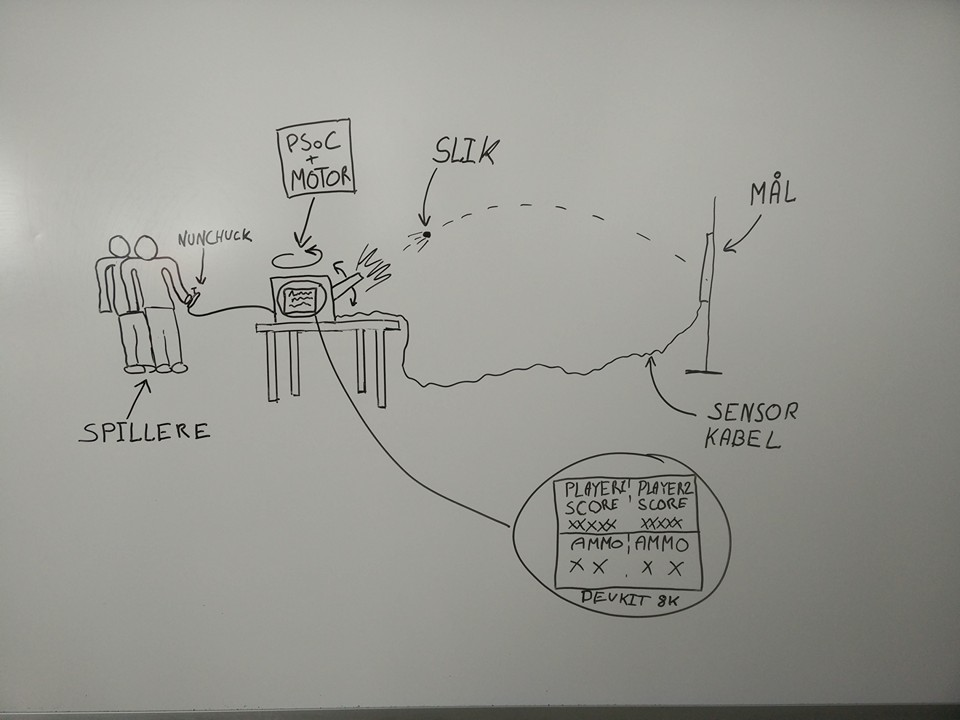
\includegraphics[width=\textwidth]{Projektformulering/images/rigtBillede}
	\caption{Rigt Billede af det endelige produkt}
	\label{ref:RigtBillede}
\end{figure}

\section{MoSCoW}
I forbindelse med projektet gøres der brug af MoSCoW-princippet for at prioritere hvilke krav, der skal være implementeret ved projektets afslutning. Ifølge MoSCoW er prioriteringerne 'Must have', 'Should have', 'Could have' og 'Won't have'. Kravene er, som følger:
\begin{itemize}
	\item{Produktet must have:}
	\subitem{En motor til styring af kanonen}
	\subitem{En brugergrænseflade til visning af statistikker}
	\subitem{En Wii-nunchuck til styring af motoren}
	\subitem{En kanon med en afskydningsmekanisme}
	\item{Produktet should have:}
	\subitem{Et mål til registering af point} 
	\subitem{En lokal ranglistestatistik}
	\item{Produktet could have:}
	\subitem{Partymode-indstilling til over to spillere}
	\subitem{Trådløs Wii-nunchuckstyring}
	\subitem{Afspilning af lydeffekter}
	\item{Produktet won't have:}
	\subitem{Et batteri til brug uden strømforsyning}
	\subitem{Online ranglistestatistik}	
\end{itemize}


\section{Opdeling af gruppen}
I løbet af projektet vil projektgruppen blive opdelt i to hovedgrupper - 'hardware' og 'software'. Disse grupper vil have til ansvar at designe og implementere hhv. hardware og software til projektet. Hardwaregruppen vil bestå af de personer, der læser til elektroingeniør (Mikkel Nielsen og Pernille Kjeldgaard). Softwaregruppen vil bestå af de personer, der læser til IKT-ingeniør (Kasper Rieder, Michael Kloock, Tenna Rasmussen, Mia Konstmann og Daniel Jensen).


